
\documentclass[crop, tikz, border=0pt]{standalone}
\usetikzlibrary{matrix}
\usetikzlibrary{patterns}
\usepackage{color}
\begin{document}
\color{white}
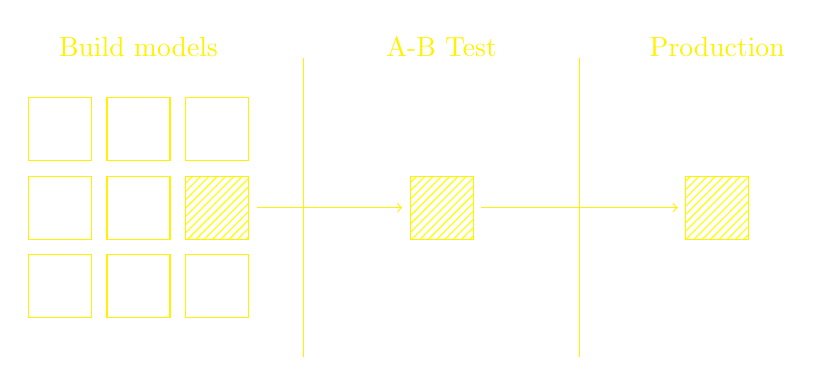
\begin{tikzpicture}[draw=yellow]
%\tikzset{rectangle node/.style = {rectangle, inner sep=1pt, draw, fill=white}}
\tikzset{edge/.style = {->,> = latex, line width=.5 pt}}

   \node[above, color=yellow] at (1.4, 3.2) {Build models};
   \foreach \x in {0,1,2}
     \foreach \y in {0,1,2}
       {\draw (\x,\y) rectangle ++(.8, .8);}
    
   \draw[yellow,pattern=north east lines, pattern color=yellow] (2,1) rectangle ++(.8, .8);    
   
   \draw  (3.5, -.5) -- (3.5, 3.3);
   
   \node[above, color=yellow] at (5.25, 3.2) {A-B Test};
   \draw[yellow,pattern=north east lines, pattern color=yellow] (4.85,1) rectangle ++(.8, .8);    
   \draw[->] (2.9, 1.4) --  (4.75, 1.4) ;
   
   \draw  (7, -.5) -- (7, 3.3); 
   
   \node[above, color=yellow] at (8.75, 3.2) {Production};
   \draw[yellow,pattern=north east lines, pattern color=yellow] (8.35,1) rectangle ++(.8, .8);
   \draw[->] (5.75, 1.4) --  (8.25, 1.4) ; 

    
\end{tikzpicture}
\end{document}